\scanpage{157}
% archive foliation: 156

\textcircled{$3'$}\quad $1,2,3$
\figure{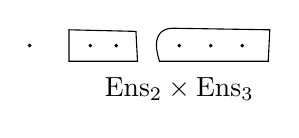
\begin{tikzpicture}[x=1cm,y=1cm]
\fill(0,0.2)circle(0.025);
\draw(0.5,0)--(0.5,0.4)--(1.35,0.38)--(1.37,0)--cycle;
\fill(0.77,0.2)circle(0.025);\fill(1.1,0.2)circle(0.025);
\draw(1.65,0)..controls(1.55,0.3)and(1.65,0.42)..(1.82,0.42)--(3.05,0.4)--(3.03,0)--cycle;
\fill(1.9,0.2)circle(0.025);\fill(2.3,0.2)circle(0.025);\fill(2.7,0.2)circle(0.025);
\node at(1.9,-0.35){$\mathrm{Ens}_2\times\mathrm{Ens}_3$};
\end{tikzpicture}}
\deleted{\unsure{biicosaèdres}}

\diagram{\begin{tikzcd}[column sep=small,row sep=small]
\textcircled{1}&(1,5)\arrow[r,leftrightarrow] &\text{(biicosaèdre)}&\\
\textcircled{2}& |[draw,ellipse]| 2,4\arrow[d,leftrightarrow,bend left=45]&
\unsure{\mathfrak G|\mathfrak S}_4\times\unsure{\mathfrak G|\mathfrak S}_2&\\
& |[draw,ellipse]| 2,2,2&
\begin{gathered}\text{i.e. cube (pas }\deleted{\unsure{\text{néc.}}}\text{ orienté)}\\
\text{ext. de }\unsure{\mathfrak G|\mathfrak S}_3\text{ par }\unsure{\mathfrak G|\mathfrak S}_2^3
\end{gathered}\arrow[r,leftrightarrow]&
\begin{gathered}\unsure{\text{en crée}}\ 2\text{ structures}\\
\text{biicos. i.e. }4\text{ str.}\\
\text{icos. formant deux}\\\text{paires d'}\unsure{\text{opposées}}\end{gathered}\\
\textcircled{3}& |[draw,ellipse]| 3,3\arrow[loop right,leftrightarrow]&
\text{ext. de }\unsure{\mathfrak G|\mathfrak S}_2\text{ par }\unsure{\mathfrak G|\mathfrak S}_3\times\unsure{\mathfrak G|\mathfrak S}_3&
\mathbf F_3^2\simeq\mathrm{Syl}_3
\end{tikzcd}}

\margin{\figure{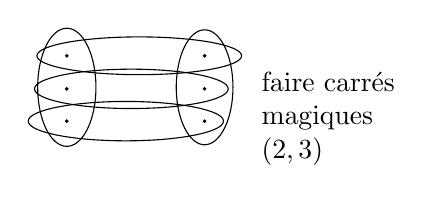
\begin{tikzpicture}[x=1cm,y=1cm]
\draw(1.3,1.05)ellipse(1.3 and .24);\draw(1.2,.63)ellipse(1.23 and .25);\draw(1.13,.22)ellipse(1.24 and .25);
\draw(.38,.65)ellipse(.37 and .75);\draw(2.13,.65)ellipse(.36 and .73);
\foreach \x in {.38,2.13}{\foreach \y in {.22,.63,1.05}{\fill(\x,\y)circle(.025);}}
\node[align=left]at(3.7,.25){faire \unsure{carrés}\\\unsure{magiques}\\$(2,3)$};
\end{tikzpicture}}}

\textcircled{$2'$}
\figure{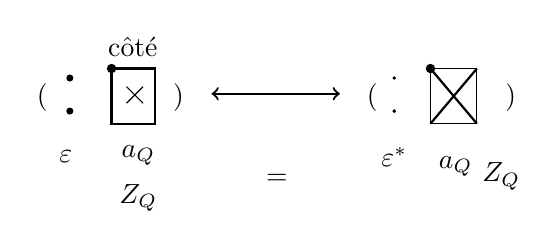
\begin{tikzpicture}[x=1cm,y=1cm]
\node at(-.35,.65){$($};\node at(1.38,.65){$)$};
\fill(0,.9)circle(.045);\fill(0,.48)circle(.045);
\node at(-.05,-.10){$\varepsilon$};
\draw[thick](.53,.32)rectangle(1.08,1.02);
\fill(.53,1.02)circle(.06);\draw(.72,.58)--(.93,.79);\draw(.72,.79)--(.93,.58);
\node at(.8,1.3){\unsure{côté}};\node at(.87,-.08){$a_Q$};\node at(.87,-.62){$Z_Q$};
\draw[<->,thick](1.80,.70)--(3.43,.70);
\node at(2.63,-.39){$=$};
\node at(3.84,.65){$($};\node at(5.60,.65){$)$};
\fill(4.12,.9)circle(.025);\fill(4.12,.48)circle(.025);
\node at(4.12,-.1){$\varepsilon^*$};
\draw(4.58,.32)rectangle(5.17,1.02);
\draw[thick](4.58,.32)--(5.17,1.02);\draw[thick](4.58,1.02)--(5.17,.32);
\fill(4.58,1.02)circle(.06);
\node at(4.9,-.22){$a_Q$};\node at(5.48,-.35){$Z_Q$};
\end{tikzpicture}}

\margin{$D_4\times\mathbf F_2\simeq\mathrm{Syl}_2$}
\[
\boxed{\begin{gathered}Q^*=\varepsilon\wedge Q^\vee\\
\deleted{\unsure{Q\simeq\varepsilon\wedge Q^*}}\end{gathered}}
\qquad\begin{gathered}\omega(Q)\simeq\omega(Q^*)=\omega\\
\deleted{\unsure{\varepsilon\wedge\varepsilon^*\wedge\omega\simeq1}}
\boxed{\varepsilon^*\wedge\varepsilon\wedge\omega\simeq1}
\end{gathered}
\]
\margin{\[
\overbrace{\varepsilon\wedge\operatorname{codiag}Q}^{\unsure{\omega(S)_6|\omega(S)}}
\simeq\overbrace{\varepsilon^*\wedge\operatorname{codiag}Q^*}^{\unsure{\omega(S^*)_6|\omega(S^*)}}
\]
i.e. $\underbrace{\varepsilon\wedge\varepsilon^*}_{\omega}\wedge
\operatorname{codiag}Q\wedge\operatorname{codiag}Q^*\simeq1$
d'où $\operatorname{codiag}Q^*\simeq\operatorname{diag}Q$}

\textcircled{$1''$}
\diagram{\begin{tikzcd}[column sep=large]
1+\text{bipentagone}\arrow[r,leftrightarrow]&1+\text{bipentagone}&\text{biicos. + sommet}\\
&\text{le }\simeq\ !&\\
1+\text{pentagone}\arrow[r,leftrightarrow]&1+\text{pentagone}&\text{icos. + sommet}
\end{tikzcd}}

\textcircled{$2''$}
\figure{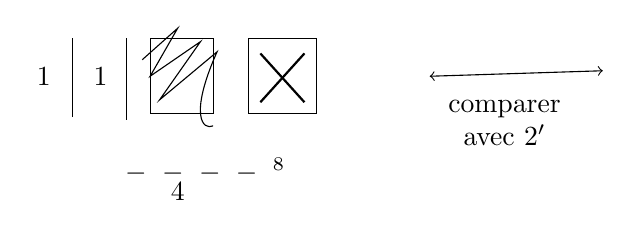
\begin{tikzpicture}[x=1cm,y=1cm]
\node at(0,.55){$1$};\draw(.36,.03)--(.36,1.03);\node at(.72,.55){$1$};\draw(1.05,0)--(1.05,1.03);
\draw(1.35,.08)rectangle(2.15,1.03);
\draw(1.25,.76)--(1.7,1.16)--(1.35,.55)--(1.99,.99)--(1.47,.25)--(2.2,.86)..controls(1.84,.05)and(2.02,-.14)..(2.15,-.08);
\draw(2.60,.08)rectangle(3.46,1.03);\draw[thick](2.75,.22)--(3.31,.84);\draw[thick](2.75,.84)--(3.31,.22);
\draw[<->](4.90,.55)--(7.10,.62);
\node[align=center]at(5.85,-.04){comparer\\avec $2'$};
\node at(2.05,-.65){$-\ -\ -\ -\ {}^8$};\node at(1.7,-.92){$\deleted{4}$};
\end{tikzpicture}}

\margin{biicos. + arête $\Vert$
\figure{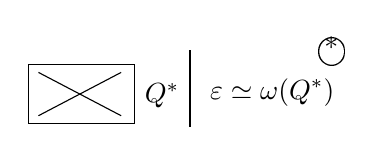
\begin{tikzpicture}[x=1cm,y=1cm]
\draw(0,0)rectangle(1.35,.75);\draw(.13,.1)--(1.18,.65);\draw(.13,.65)--(1.18,.1);
\node at(1.70,.36){$Q^*$};\draw[thick](2.05,-.04)--(2.05,.94);
\node at(3.1,.4){$\varepsilon\simeq\omega(Q^*)$};\node at(3.85,.92){$\textcircled{*}$};
\end{tikzpicture}}
icos. + arête \deleted{$\unsure{\varepsilon}$}
\figure{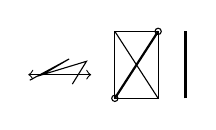
\begin{tikzpicture}[x=1cm,y=1cm]
\draw[<->](0,.3)--(.8,.3);\draw(.02,.23)--(.52,.5)--(.18,.3)--(.74,.47)--(.56,.18);
\draw(1.1,0)rectangle(1.65,.85);\draw[thick](1.1,0)--(1.65,.85);\draw(1.1,.85)--(1.65,0);
\draw(1.1,0)circle(.04);\draw(1.65,.85)circle(.04);\draw[very thick](2,0)--(2,.85);
\end{tikzpicture}}}

\textcircled{$3''$}
\figure{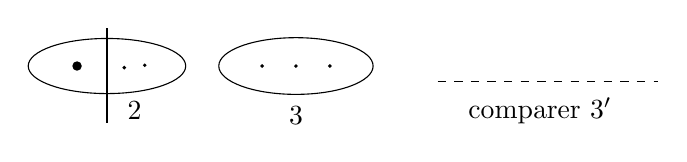
\begin{tikzpicture}[x=1cm,y=1cm]
\draw(1,.60)ellipse(1 and .35);\fill(.62,.6)circle(.06);\fill(1.22,.58)circle(.025);\fill(1.48,.61)circle(.025);
\draw(1,-.12)--(1,1.08);\node at(1.35,.04){$2$};
\draw(3.4,.60)ellipse(.98 and .36);\foreach\x in{2.97,3.4,3.83}{\fill(\x,.6)circle(.025);}\node at(3.4,-.03){$3$};
\draw[dashed](5.2,.4)--(8,.4);\node at(6.5,.03){comparer $3'$};
\end{tikzpicture}}
\deleted{$\unsure{a\ a'\ a\ v',\ b\ u'}$}

\margin{biicos. + biface \unsure{un prisme}
\figure{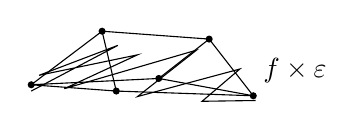
\begin{tikzpicture}[x=1cm,y=1cm]
\coordinate(A)at(0,0);\coordinate(B)at(.9,.68);\coordinate(C)at(1.08,-.08);
\coordinate(D)at(1.62,.08);\coordinate(E)at(2.26,.58);\coordinate(F)at(2.82,-.14);
\draw(A)--(B)--(C)--cycle;\draw(D)--(E)--(F)--cycle;\draw(A)--(D);\draw(B)--(E);\draw(C)--(F);
\foreach\p in{A,B,C,D,E,F}{\fill(\p)circle(.045);}
\draw(0,-.08)--(1.1,.5)--(.1,.12)--(1.35,.38)--(.42,-.05)--(2.1,.44)--(1.35,-.15)--(2.65,.2)--(2.17,-.21)--(2.85,-.2);
\node at(3.35,.18){$f\times\varepsilon$};
\end{tikzpicture}}
icos + face\quad \unsure{un prisme}\quad $f\times\{0,1\}$}

\figure{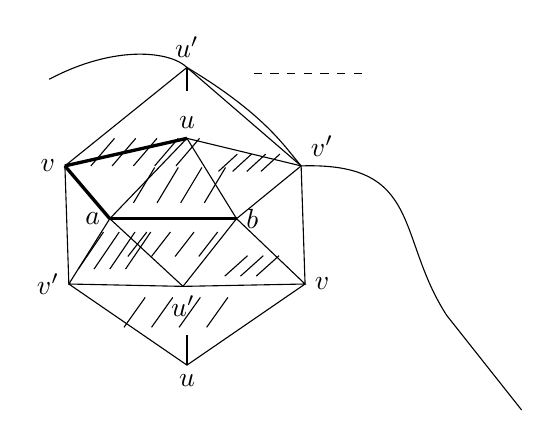
\begin{tikzpicture}[x=1cm,y=1cm]
\coordinate(T)at(2,3.8);\coordinate(U)at(2,2.9);\coordinate(L)at(.45,2.55);\coordinate(R)at(3.45,2.55);
\coordinate(A)at(1.02,1.88);\coordinate(B)at(2.63,1.88);\coordinate(LL)at(.50,1.05);\coordinate(RR)at(3.50,1.05);
\coordinate(UU)at(1.95,1.02);\coordinate(BT)at(2,.02);
\draw(T)--(L)--(LL)--(BT)--(RR)--(R)--cycle;
\draw(L)--(U)--(R);\draw(L)--(A)--(U)--(B)--(R);\draw(A)--(LL)--(UU)--(RR)--(B);\draw(A)--(UU)--(B);\draw(A)--(B);
\draw[very thick](L)--(U);\draw[very thick](L)--(A);\draw[very thick](A)--(B);
\foreach\x in{.78,1.05,1.32,1.59,1.86}{\draw(\x,2.55)--++(.30,.35);}
\foreach\x in{1.32,1.62,1.92,2.22}{\draw(\x,2.08)--++(.27,.45);}
\foreach\x in{2.40,2.58,2.76,2.94}{\draw(\x,2.48)--++(.24,.22);}
\foreach\x in{.62,.82,1.02,1.22}{\draw(\x,1.24)--++(.32,.47);}
\foreach\x in{1.25,1.55,1.85,2.15}{\draw(\x,1.40)--++(.24,.31);}
\foreach\x in{2.48,2.68,2.88}{\draw(\x,1.15)--++(.29,.26);}
\foreach\x in{1.20,1.55,1.90,2.25}{\draw(\x,.50)--++(.27,.38);}
\draw(T)--++(0,-.3);\draw(BT)--++(0,.38);
\node[above]at(T){$u'$};\node[above]at(U){$u$};\node[left]at(L){$\unsure{v}$};\node[above right]at(R){$v'$};
\node[left]at(A){$a$};\node[right]at(B){$b$};\node[left]at(LL){$v'$};\node[right]at(RR){$v$};\node[below]at(UU){$u'$};\node[below]at(BT){$u$};
\draw(.25,3.65)..controls(1.1,4.1)and(1.8,4.0)..(T)..controls(3,3.2)and(3.25,2.78)..(R)
..controls(5,2.60)and(4.65,1.65)..(5.30,.65)--(6.25,-.55);
\draw[dashed](2.85,3.72)--(4.25,3.72);
\end{tikzpicture}}

\unsure{Programme :} icosaèdre

\diagram{\begin{tikzcd}
\{a,b\}\wedge\{u,u'\}\arrow[r]&\{v,v'\}
\end{tikzcd}}
\deleted{$\unsure{\{a,b\}\wedge u}$}\qquad $a\wedge u=v$
\[
a\wedge v=u'
\]
\[
\{a,b\}\wedge
\underset{\operatorname{codiag}(Q)}{\underbrace{\{u,u'\}}\wedge\underbrace{\{v,v'\}}}
\simeq\deleted{\unsure{\omega(S)}}\operatorname{diag}Q
\]
\[
\{a\unsure{\wedge|,}b\}\simeq\omega(Q)
\]

\margin{\textcircled{*} choix d'une structure icosaédrale du
\unsure{G} biicosaèdre
$\simeq\operatorname{diag}(Q)$ / \unsure{Mais on}
$\simeq\unsure{\omega_\Delta|\omega}(S\amalg\varepsilon)
\simeq\omega(S)\wedge\varepsilon\simeq\operatorname{codiag}(Q)\wedge\varepsilon
\simeq\operatorname{diag}Q$ OK!}
